\begin{figure}[h]
	\centering
	\begin{subfigure}[h!]{0.3\textwidth}
		\centering
		\begin{minipage}{4cm}
			\begin{Verbatim}[commandchars=\\\{\}]
x = \textcolor{red}{"a"}
while ...
    x = \textcolor{red}{"["} x \textcolor{red}{"]"}
print x
			\end{Verbatim}
		\end{minipage}
		\caption{Код}
		\label{fig:code}
	\end{subfigure}
	~
	\begin{subfigure}[h!]{0.3\textwidth}
		\centering
		$
		\begin{array}{crcl}
			&s' &::=& s \\
			&s & ::= & \mbox{\texttt{LBR }} s \mbox{\texttt{ RBR}}\\
			&s & ::= & \mbox{\texttt{A}}
		\end{array}
		$
		\caption{КС-аппроксимация}
		\label{fig:app_cf}
	\end{subfigure}
	~
	\begin{subfigure}[h!]{0.3\textwidth}
		\centering
		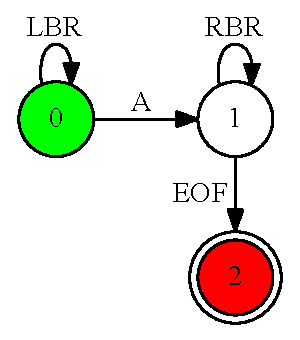
\includegraphics[width=2.5cm]{pictures/reg_app}
		\caption{Регулярная}
		\label{fig:app_r}
	\end{subfigure}
	\caption{Исходный код и примеры аппроксимаций}
	\label{example}
\end{figure}